\chapter{Application}\label{chap:application}
In order to create a robust system, two solutions are proposed. The first utilizes the fact that a person faces 
the same direction their waist faces. So we create a plane between three fixed 
points, the center hip $\vec{c}$, the left $\vec{l}$ and the right hips $\vec{r}$. A normal vector \N was created 
from this plane in order to allow the program to recognize where the person is 
facing. 
\\
\\
\centerline{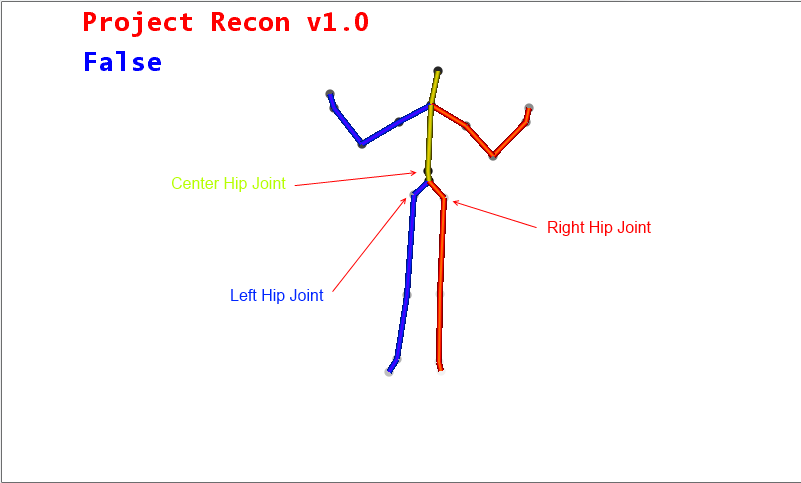
\includegraphics[scale=0.5]{skeleton_frame3.png}}
\centerline{fig.4.6 (In the figure the three joints are pointed out and named)}
\\
\\
To calculate the normal vector, we subtract the right and left hip joints from 
the center hip joint and then we calculate the cross product of the two 
subtractions.
\\
\\
\N = ($\vec{r}$ - $\vec{c}$) X ($\vec{l} - \vec{c}$)
\\
\\
We then calculate the normal by using the Normalize method.
\begin{verbatim}
var dir = Vector3.Cross(rhip - chip, lhip - chip);
var norm = Vector3.Normalize(dir);
\end{verbatim}
As the person turns, the normal vector will be used as a reference to calculate the angle between it and the Z axis. This will allow us to rotate the skeleton so that it will be always facing the Kinect. Recognition will then take place.
\\
\\
Kinect has another problem, which is that it cannot diffrentiate between a user giving it his face or his back. In other words, a user's left and right are swaped if the user is giving the Kinect his back.

%put an image to make it better understandable

The normal vector calculation approach will reswap the left joints with the right joints when the \N is on the negative Z axis. 
However, here another problem emerges. When the swap takes place, an error occurs. Mainly, the programmer can not 
edit the value of the position of the joints. The value is read from the skeleton 
stream of the Kinect. In order to resolve this, an avatar skeleton needs to be 
created, littleGuy. littleGuy is an array of SkeletonPoints, where every 
SkeletonPoint represents a joint, and gets the value from these joints. This 
helps in allowing us to edit and the SkeletonPoints as we wish and in the end 
draw this avatar skeleton instead.
\\
\\
In the figure below the user is facing their right, having the normal vector (red 
line) erected and defining the direction the user is facing.
\\
\\
\centerline{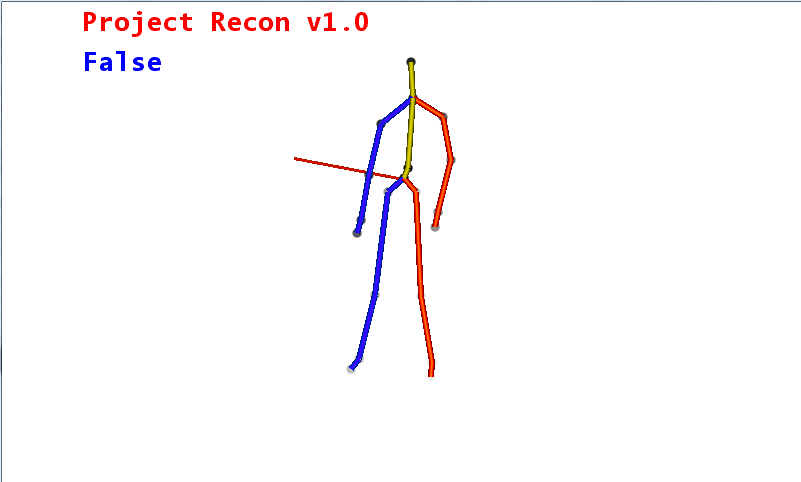
\includegraphics[scale=0.5]{skeleton_normal.png}}
\\
\centerline{fig.4.6 (Skeleton with a normal vector defining where it is facing)}
\\
\\
%talk about the problem in the kinect sensor and recognizing the different side of the skeleton 
The second solution is using Kinect's face detection capabilities, which may be 
hard and require high processing. More research is needed in this part to better 
understand it.
%here talk about the final way and discuss how you will use the recognition to solve the issue with robustness
\section{Recognition}
Recognition is the essence of this project. Recognition needs to be in real time, but most importantly how will the recognition occur. We discussed in the previous section the resolve of the normal vector. However, why is it needed? In recognition we want to be able to translate the skeleton of the person in order to always recognize from the same direction, facing the Kinect. In the coming sections we will discuss the different ways for recognition.
\subsection{Glyphs Method}
\subsection{Frames}